\documentclass[a4paper,12pt]{article}[abntex2]
\bibliographystyle{abntex2-alf}
\usepackage[table,xcdraw]{xcolor}

% Definições de layout e formatação
\usepackage[a4paper, left=3.0cm, top=3.0cm, bottom=2.0cm, right=2.0cm]{geometry} % Personalização das margens do documento
\usepackage{setspace} % Controle do espaçamento entre linhas
\onehalfspacing % Espaçamento entre linhas de 1,5
\usepackage{indentfirst} % Indentação do primeiro parágrafo das seções
\usepackage{newtxtext} % Substitui a fonte padrão pela Times Roman
\usepackage{titlesec} % Personalização dos títulos de seções
\usepackage{ragged2e} % Melhor controle de justificação do texto
\usepackage[portuguese]{babel} % Adaptação para o português (nomes e hifenização)
\usepackage{amsmath}

% Pacotes de cabeçalho, rodapé e títulos
\usepackage{fancyhdr} % Customização de cabeçalhos e rodapés
\setlength{\headheight}{14.49998pt} % Altura do cabeçalho
\pagestyle{fancy}
\fancyhf{} % Limpa cabeçalho e rodapé
\rhead{\thepage} % Página no canto direito do cabeçalho

% Pacotes para tabelas
\usepackage{booktabs} % Melhora a qualidade das tabelas
\usepackage{tabularx} % Permite tabelas com larguras de colunas ajustáveis
\usepackage{float} % Melhor controle sobre o posicionamento de figuras e tabelas

% Pacotes para gráficos e imagens
\usepackage{graphicx} % Suporte para inclusão de imagens

\usepackage[utf8]{inputenc}
\usepackage{listingsutf8}

\lstset{
    language=R,                      
    basicstyle=\ttfamily\scalefont{1.0},
    keywordstyle=\color{blue},       
    stringstyle=\color{red},         
    commentstyle=\color{green},      
    numbers=left,                    
    numberstyle=\tiny\color{gray},   
    stepnumber=1,                    
    numbersep=5pt,                   
    backgroundcolor=\color{lightgray!10}, 
    frame=single,                    
    breaklines=true,                 
    captionpos=b,                    
    keepspaces=true,                 
    showspaces=false,                
    showstringspaces=false,          
    showtabs=false,                  
    tabsize=2,
     literate={á}{{\'a}}1
             {é}{{\'e}}1
             {í}{{\'i}}1
             {ó}{{\'o}}1
             {ú}{{\'u}}1
             {Ú}{{\'U}}1
             {â}{{\^a}}1
             {ê}{{\^e}}1
             {î}{{\^i}}1
             {ô}{{\^o}}1
             {û}{{\^u}}1
             {ã}{{\~a}}1
             {õ}{{\~o}}1
             {ç}{{\c{c}}}1,
}


% Pacotes para unidades e formatação numérica
\usepackage{siunitx} % Tipografia de unidades do Sistema Internacional e formatação de números
\sisetup{
  output-decimal-marker = {,},
  inter-unit-product = \ensuremath{{}\cdot{}},
  per-mode = symbol
}
\DeclareSIUnit{\real}{R\$}
\newcommand{\real}[1]{R\$#1}

% Pacotes para hiperlinks e referências
\usepackage{hyperref} % Suporte a hiperlinks
\usepackage{footnotehyper} % Notas de rodapé clicáveis em combinação com hyperref
\hypersetup{
    colorlinks=true,
    linkcolor=black,
    filecolor=magenta,      
    urlcolor=cyan,
    citecolor=black,        
    pdfborder={0 0 0},
}
\makeatletter
\def\@pdfborder{0 0 0} % Remove a borda dos links
\def\@pdfborderstyle{/S/U/W 1} % Estilo da borda dos links
\makeatother

% Pacotes para texto e outros
\usepackage{lipsum} % Geração de texto dummy 'Lorem Ipsum'
\usepackage[normalem]{ulem} % Permite o uso de diferentes tipos de sublinhados sem alterar o \emph{}

\begin{document}

\begin{titlepage}
    \centering
    \vspace*{1cm}
    \Large\textbf{INSPER – INSTITUTO DE ENSINO E PESQUISA}\\
    \Large ECONOMIA\\
    \vspace{1.5cm}
    \Large\textbf{Atividade Prática Supervisionada - APS}\\
    \textbf{Comércio Internacional}\\
    \vspace{1.5cm}
    Prof. Arthur Augusto Viaro\\
    \vfill
    \normalsize
    Érika Kaori Fuzisaka, \href{mailto:erikakf1@al.insper.edu.br}{erikakf1@al.insper.edu.br}\\
    Hicham Munir Tayfour, \href{mailto:hichamt@al.insper.edu.br}{hichamt@al.insper.edu.br}\\

    \vfill
    São Paulo\\
    Abril/2025
\end{titlepage}

\newpage
\tableofcontents
\thispagestyle{empty} % Esse comando remove a numeração de pagina da tabela de conteúdo

\newpage 
\listoffigures
\thispagestyle{empty} % Esse comando remove a numeração de pagina da tabela de figura

\newpage
\listoftables
\thispagestyle{empty} % Este comando remove a numeração de página da lista de tabelas

\newpage
\setcounter{page}{1} % Inicia a contagem de páginas a partir desta página
\justify
\onehalfspacing

\section*{\textbf{Resumo executivo}}
\addcontentsline{toc}{section}{Resumo executivo}

As novas tarifas americanas (10–50\% sobre mais de 180 países) tendem a encarecer bens importados, reduzir variedade disponível e realocar fatores para setores menos eficientes.  
Curto prazo, ramos protegidos ganham margem, mas consumidores e indústrias que usam insumos estrangeiros perdem.  
Longo prazo, capital e trabalho migram: salários reais de trabalhadores pouco qualificados caem, retorno do capital sobe e a produtividade desacelera.  
Externamente, exportadores intensivos em trabalho sofrem com a queda de demanda, cadeias globais se fragmentam e cresce o risco de retaliação.

\section*{\textbf{Cenário Atual}}
\addcontentsline{toc}{section}{Cenário Atual}

Nas últimas semanas, a decisão do governo dos EUA de implementar tarifas comerciais recíprocas sobre produtos de mais de 180 países, com alíquotas variando entre 10\% e 50\%, reacendeu o debate global sobre impactos do protecionismo no comércio internacional. Um cenário de crescente interdependência econômica, essa medida levanta questionamentos sobre seus efeitos nos consumidores, produtores, trabalhadores e na dinâmica política e econômica tanto nos EUA quanto no restante do mundo. Este memorando tem como objetivo analisar possíveis consequências dessa política tarifária, usando teorias econômicas consolidadas e evidências empíricas, a fim de informar o público geral e contribuir para um debate sobre o tema.

\section*{\textbf{Impacto sobre consumidores}}
\addcontentsline{toc}{section}{Impacto sobre consumidores}

\subsection*{\textbf{EUA}}
\addcontentsline{toc}{subsection}{EUA}

Sob o \textbf{modelo ricardiano}, as tarifas elevam o preço interno dos bens importados; a linha orçamentária se torna mais horizontal, reduzindo o conjunto de cestas acessíveis e, portanto, o bem-estar. A Figura~\ref{fig:budget} ilustra essa rotação. Essa rotação transforma parte da renda do consumidor em receita de imposto e gera perda líquida de bem-estar. 

\begin{figure}[H]
  \centering
  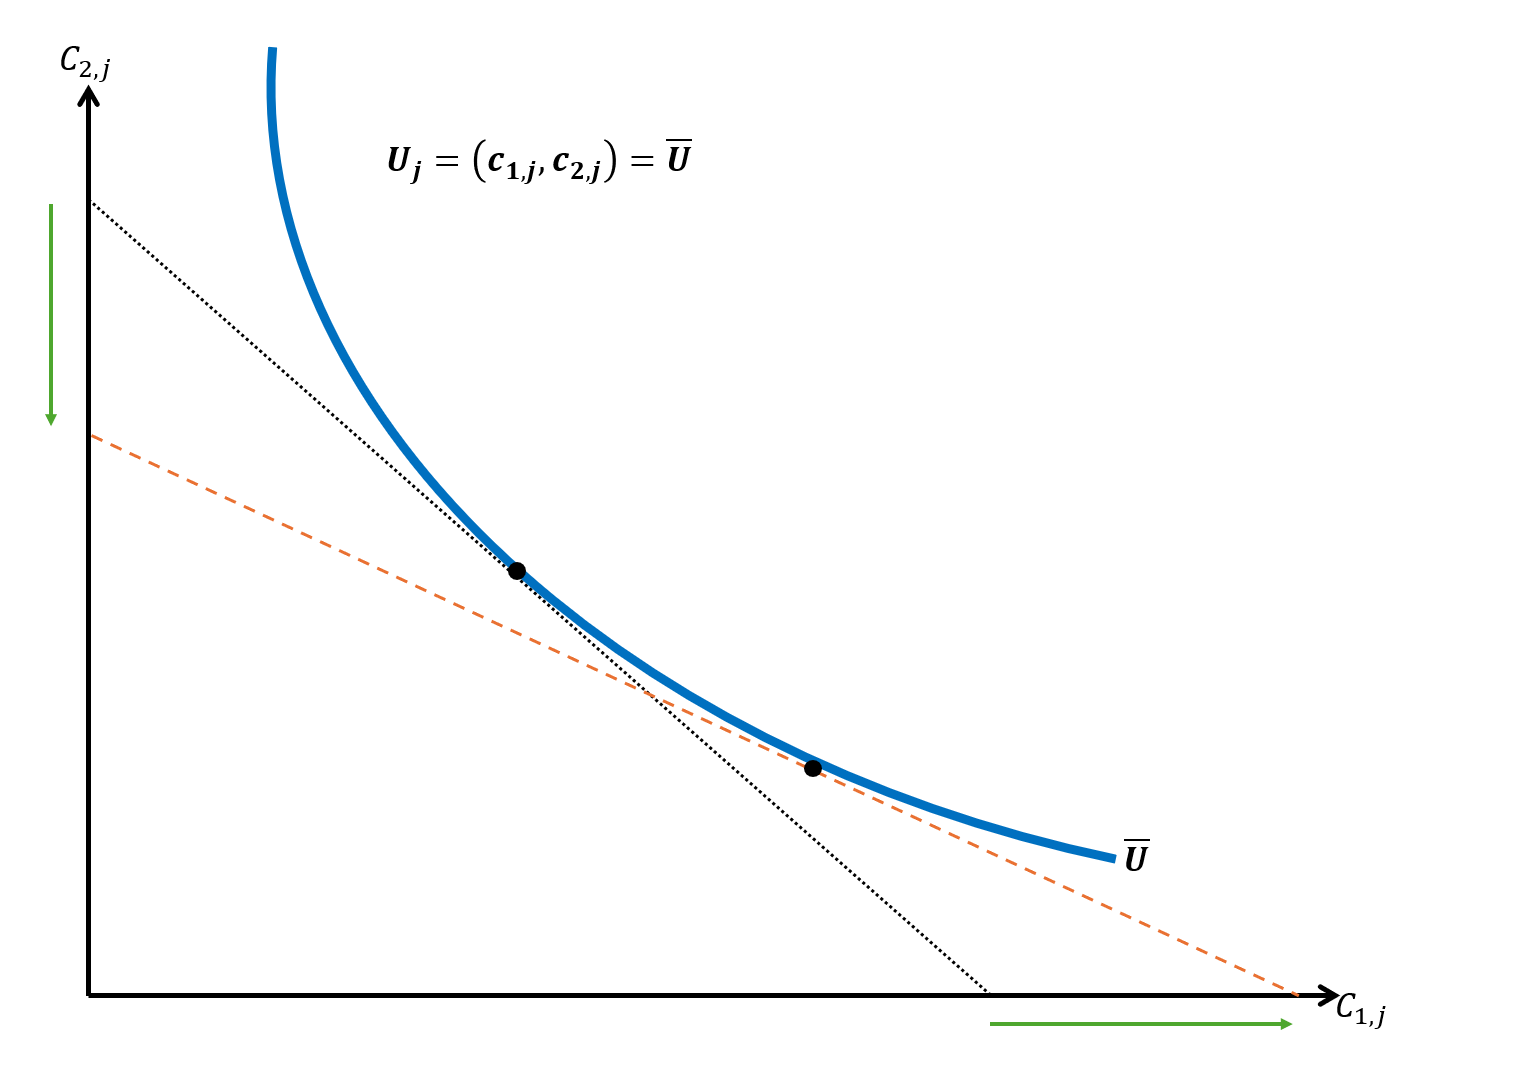
\includegraphics[width=0.7\linewidth]{Imagens/aps1i1.png}
  \caption{Rotação da restrição orçamentária dos consumidores dos EUA após tarifa.}
  \label{fig:budget}
\end{figure}

Pela lógica de \textbf{Krugman} (economias de escala e competição monopolística), quando a tarifa encarece o acesso ao mercado, parte das firmas estrangeiras sai dos EUA; cai o número de variedades disponíveis ($n\downarrow$). Com menos concorrência, as empresas que ficam aumentam sua margem de lucro, comprimindo ainda mais o excedente do consumidor (\emph{love for variety}).

\begin{equation}
p_i' = (1+\tau) \cdot p_i
\end{equation}

No curtíssimo prazo não há substitutos domésticos suficientes; consumidores simplesmente pagam mais. Com o tempo, fabricantes locais podem expandir a oferta, mas a literatura empírica mostra que a queda de preços raramente compensa totalmente a perda inicial de bem-estar.

\subsection*{\textbf{Resto do Mundo}}
\addcontentsline{toc}{subsection}{Resto do Mundo}

\begin{enumerate}
    \item \textbf{Em países afetados diretamente pelas tarifas}\\
    O desvio de demanda dos EUA cria excedente interno, pressionando o preço doméstico desses países \emph{para baixo}.  
    Para o consumidor local, isso significa pagar menos pelo menos no curto prazo. O mecanismo é o mesmo descrito no modelo Heckscher-Ohlin: um choque negativo no preço relativo do bem exportado se traduz em queda de preço interno e ganho imediato de excedente para quem compra.

    \item \textbf{Em países não-alvo, mas que podem abastecer o mercado norte-americano}\\
    O efeito é mais tênue. Alguns produtores desviam vendas para atender o mercado interno dos EUA, reduzindo a oferta interna, portanto eleva um pouco o preço local desses bens. Por outro lado, a pressão de baixa sobre o preço mundial de determinadas commodities também chega aos consumidores e pode contrabalançar esse movimento. Para o consumidor médio, o saldo costuma oscilar pouco, não uma alta generalizada. A teoria gravitacional de comércio sugere que o maior impacto nem é no preço, mas no custo logístico: tarifas e incerteza regulatória elevam frete e prazos, e parte disso é repassada ao varejo.

    \item \textbf{No mundo todo (efeito de variedade e mark-up)}\\
    Mesmo onde os preços movem pouco, uma perda "silenciosa" é notada: menor variedade de produtos e margens maiores para produtos diferenciados. O modelo de economias de escala com concorrência monopolística (Krugman) mostra que, quando o maior mercado mundial encolhe, o número mundial de variedades viáveis diminui; com menos concorrência, as empresas restantes elevam seus mark-ups. Resultado: opções mais limitadas e aumentos em itens de nichos diferenciados (como vinhos, cosméticos, eletrônicos premium).
\end{enumerate}

\section*{\textbf{Impacto sobre os Produtores}}
\addcontentsline{toc}{section}{Impacto sobre os Produtores}

\subsection*{\textbf{Curto prazo}}
\addcontentsline{toc}{subsection}{Curto Prazo}

\begin{itemize}
  \item \textbf{EUA} – Nos setores protegidos (como aço, alumínio), o preço de venda sobe assim que a tarifa entra em vigor. Com o capital ainda \emph{específico} ao setor, as margens aumentam e parte desse ganho reflete em salários setoriais maiores, como previsto no modelo de \textit{Fatores Específicos}. Já firmas que dependem de insumos importados veem seus custos crescerem e perdem competitividade interna e externa.

  \item \textbf{Resto do mundo} – Exportadores que abasteciam o mercado estadunidense perdem pedidos imediatamente, gerando capacidade ociosa. O excedente é desviado para mercados domésticos ou terceiros países a preços menores, comprimindo margens. Concorrentes diretos dos EUA em mercados de terceiros podem ganhar volume, mas sob preços deprimidos.
\end{itemize}

\subsection*{\textbf{Longo prazo}}
\addcontentsline{toc}{subsection}{Longo prazo}

\begin{itemize}
  \item \textbf{EUA} – Com fatores de produção móveis, vale o Teorema de Rybczynski: insistir em bens intensivos em trabalho num país relativamente abundante em capital leva a uso ineficiente de recursos. A rentabilidade cai, parte do capital migra para setores não tarifados ou para o exterior, portanto a produtividade agregada recua. A proteção prolongada reduz incentivos à inovação; quando a concorrência externa diminui, o "bônus" inicial converge para zero à medida que cadeias globais se ajustam.
  
  \item \textbf{Resto do mundo} – As Firmas estrangeiras podem reagir de três maneiras: 
  \begin{enumerate}
    \item instalam unidades nos EUA para contornar a tarifa, arcando com custos maiores; 
    \item redirecionam vendas a novos mercados (América Latina, UE, Ásia); ou 
    \item escalam na cadeia de valor, oferecendo bens diferenciados. 
  \end{enumerate}
  
  Ainda assim, a contração do maior mercado mundial reduz a escala eficiente global e o número de variedades lucrativas, como o modelo de Krugman indica.
\end{itemize}

\section*{\textbf{Impacto sobre Trabalhadores}}
\addcontentsline{toc}{section}{Impacto sobre Trabalhadores}

\subsection*{\textbf{EUA}}
\addcontentsline{toc}{subsection}{Trabalhadores nos EUA}

\begin{itemize}
  \item \textbf{Setores protegidos} 
  \begin{itemize}
    \item \textbf{No curto prazo:} Pós choque, setores como aço, alumínio, têxteis e ramos semelhantes vendem mais no mercado doméstico. A receita cresce e as empresas buscam operários adicionais; salários nominais sobem porque capital e equipamentos não conseguem mudar de setor de um dia para o outro (mecanismo do modelo de Fatores Específicos).
    
    \item \textbf{No médio prazo:} Parte do ganho nominal é consumida pela inflação gerada pela própria tarifa. Ainda assim, esses trabalhadores preservam alguma vantagem, pois a demanda interna continua deslocada a favor dos bens protegidos.
    
    \item \textbf{No longo prazo:} Uma vez que capital e trabalho passam a circular entre setores, vigora a lógica Stolper-Samuelson: o bem trabalho-intensivo segue relativamente caro e o salário real do operário menos qualificado permanece acima do que estaria sem a tarifa. Porém, quando a proteção se torna crônica, a menor concorrência externa reduz investimentos em P\&D; no quadro de longo prazo descrito por Krugman, a menor variedade e os mark-ups mais altos derrubam o crescimento de produtividade, limitando avanços salariais futuros.
  \end{itemize}
  
  \item \textbf{Demais setores} 
  \begin{itemize}
    \item \textbf{No curto prazo:} Indústrias que dependem de insumos importados como montadoras e de eletrônicos enfrentam dificuldades. Para defender margens, congelam salários, suspendem horas extras ou demitem. O encarecimento dos bens de consumo eleva o custo de vida, de modo que o salário real cai para a maioria dos trabalhadores fora dos setores protegidos.
    
    \item \textbf{No médio prazo:} Empresas afetadas tentam redesenhar cadeias de suprimento, automatizar processos ou mesmo transferir parte da produção para o exterior. Empregos de qualificação intermediária encolhem; cresce a procura por profissionais de logística e de compras internacionais.
    
    \item \textbf{No longo prazo:} O retorno do capital fica menor e o salário dos qualificados avança menos do que avançaria num cenário de livre-comércio; toda a economia sente o freio no ganho de produtividade que decorre de menos variedade e menos escala.
  \end{itemize}
\end{itemize}

\subsection*{\textbf{Resto do mundo}}
\addcontentsline{toc}{subsection}{Resto do mundo}

\begin{itemize}
  \item \textbf{Exportadores diretamente afetados} 
  \begin{itemize}
    \item \textbf{No curto prazo:} Nos países que vendiam intensivamente para o mercado norte-americano, pedidos caem, turnos são reduzidos e salários nominais recuam nos setores atingidos.
    
    \item \textbf{No médio prazo:} Parte desses trabalhadores é realocada para vender em mercados alternativos, mas costuma receber salários menores; outras plantas fecham por falta de escala.
    
    \item \textbf{No longo prazo:} A retração permanente do maior mercado consumidor faz a produtividade global crescer mais devagar; salários reais nesses países ficam abaixo da trajetória que seguiriam sem a tarifa.
  \end{itemize}
  
  \item \textbf{Países terceiros que recebem desvio de comércio} 
  \begin{itemize}
    \item \textbf{No curto prazo:} Em países que substituem parcialmente as vendas aos EUA, alguns ramos contratam mais e pagam salários um pouco maiores, mas o efeito é restrito a nichos específicos.
    
    \item \textbf{No médio e longo prazos:} Quando a contração do mercado americano reduz o tamanho mínimo eficiente das cadeias globais, até esses ganhos pontuais desaparecem; o crescimento salarial desacelera de maneira generalizada, sobretudo em economias abundantes em mão-de-obra.
  \end{itemize}
\end{itemize}

\section*{\textbf{Considerações Políticas}}
\addcontentsline{toc}{section}{Considerações Políticas}

\subsection*{\textbf{Grupos domésticos que tendem a apoiar}}
\addcontentsline{toc}{subsection}{Grupos domésticos que tendem a apoiar}

\begin{itemize}
    \item \textbf{Indústrias intensivas em trabalho pouco qualificado} (como siderurgia e metalurgia básica): concentram ganhos claros de curto prazo — preços de venda e retorno do capital específico aumentam.  
    \item \textbf{Sindicatos de setores protegidos}: veem a tarifa como mecanismo de preservar e elevar empregos na manufatura tradicional. 
    \item \textbf{Eleitores populistas/nacionalistas} que associam déficit comercial a perda de "grandeza" econômica ou segurança nacional.
\end{itemize}

\subsection*{\textbf{Grupos domésticos que tendem a se opor}}
\addcontentsline{toc}{subsection}{Grupos domésticos que tendem a se opor}

\begin{itemize}
    \item \textbf{Setores intensivos em importações} (automóveis, eletrônicos, construção): margens comprimem-se quando o custo de insumos estrangeiros sobe.  
    \item \textbf{Varejo de grande escala} e \textbf{empresas de e-commerce}: dependem de bens de consumo importados de baixo custo; repassem de preço atinge consumidores.  
    \item \textbf{Agronegócio e indústrias exportadoras}: temem retaliação estrangeira que feche mercados ou imponha quotas.  
    \item \textbf{Consumidores urbanos} e organismos pró-mercado que valorizam preços baixos e variedade; percebem o imposto oculto da tarifa.
\end{itemize}

\subsection*{\textbf{Possíveis repercussões internacionais}}
\addcontentsline{toc}{subsection}{Possíveis repercussões internacionais}

\begin{enumerate}
    \item \textbf{Retaliação tarifária} — parceiros afetados (UE, China, México, Canadá) podem impor tarifas equivalentes sobre exportações dos EUA, sobretudo em bens agrícolas e manufaturas politicamente sensíveis.  
    \item \textbf{Disputas na OMC} — países recorrerão ao mecanismo de solução de controvérsias; demora de anos aprofunda incerteza regulatória.  
    \item \textbf{Erosão da credibilidade multilateral} — a medida incentiva acordos regionais ou bilaterais que excluam os EUA, fortalecendo alianças comerciais alternativas (RCEP, UE e Mercosul).  
    \item \textbf{Escalada protecionista} — outros governos podem usar o precedente para justificar barreiras "recíprocas", elevando o custo global de comércio e fragmentando cadeias de valor.  
    \item \textbf{Repercussões geopolíticas} — aliados tradicionais questionam o compromisso dos EUA com normas internacionais; rivais estratégicos (China) aproveitam o vácuo para projetar liderança em comércio e investimento.
\end{enumerate}

\section*{\textbf{Impacto Macroeconômico e Países Mais Afetados}}
\addcontentsline{toc}{section}{Impacto Macroeconômico e Países Mais Afetados}

\subsection*{\textbf{EUA}}
\addcontentsline{toc}{subsection}{EUA}

Do ponto de vista da teoria, as tarifas levam a economia norte-americana para fora da sua vantagem comparativa. Nos modelos referenciados, um país relativamente abundante em capital, como os EUA, torna-se menos eficiente quando passa a produzir bens mais intensivos em trabalho que antes importava. Essa realocação faz a fronteira de possibilidades de consumo recuar e reduz o bem-estar agregado. 

No curto prazo, o modelo de fatores específicos ajuda a entender por que os setores protegidos inicialmente prosperam: o preço doméstico dos seus produtos sobe enquanto o capital permanece preso ao setor, elevando lucros e salários locais. Entretanto, consumidores e indústrias que dependem de insumos importados enfrentam preços mais altos, de modo que o ganho concentrado desses ramos não compensa o "imposto" espalhado pelo resto da economia. 

Quando se consideram as economias de escala descritas por Krugman, a situação piora: a redução de importações diminui a variedade disponível, encolhe a escala ótima de produção e eleva as margens de monopólio, o que prejudica a produtividade total dos fatores. Em conjunto, esses mecanismos apontam para um leve recuo do PIB real, inflação de bens protegidos e queda na eficiência produtiva doméstica.

\subsection*{\textbf{Resto do mundo}}
\addcontentsline{toc}{subsection}{Resto do mundo}

No exterior, a lógica se inverte. Países abundantes em trabalho (tipicamente exportadores de bens intensivos nesse fator) perdem parte da demanda no item em que são mais eficientes, que deprime o preço relativo do produto e reduz salários reais. Com capital e trabalhadores específicos a esse setor, a queda de receita se traduz em cortes de emprego e deslocamento de mão de obra para atividades menos produtivas. 

Além disso, a contração do maior mercado consumidor do mundo reduz o número de variedades globalmente rentáveis, comprimindo a escala das plantas industriais e, por consequência, a produtividade mundial. O modelo de competição monopolística mostra que esse efeito de menor variedade gera perda de bem-estar mesmo para países que não são alvo direto das tarifas.

As tarifas reduzem a eficiência dentro dos EUA, retiram renda dos exportadores mais dependentes do mercado norte-americano e, ao fragmentar as cadeias globais, impõem um custo de menor escala e menor produtividade da economia mundial.

\section*{\textbf{Conclusão}}
\addcontentsline{toc}{section}{Conclusão}

Através das principais teorias de comércio e da evidência empírica, as tarifas recíprocas \textbf{diminuem o bem‑estar agregado}, beneficiam grupos específicos às custas de consumidores e produtores integrados a cadeias globais, e alimentam retaliações que erodem a posição dos EUA no sistema multilateral. 

Políticas alternativas de apoio à competitividade — qualificação de trabalhadores e inovação —oferecem custo‑benefício superior sem comprometer os \textit{ganhos de troca} que sustentam o crescimento global.


\end{document}
